% !TEX program = xelatex
\documentclass[11pt,a4paper]{ctexart}
\usepackage{amsmath,amssymb}
\usepackage[margin=1.65cm,top=1.5cm,bottom=1.6cm]{geometry}
\usepackage{enumitem}
\usepackage{tabularx}
\usepackage{graphicx}
\usepackage{xcolor}
\usepackage{fancyhdr}

\pagestyle{fancy}
\fancyhf{}
\renewcommand{\headrulewidth}{0pt}
\renewcommand{\footrulewidth}{0pt}
\fancyfoot[C]{\small\thepage}
\fancypagestyle{plain}{\fancyhf{}\renewcommand{\headrulewidth}{0pt}\fancyfoot[C]{\small\thepage}}

\setlength{\parindent}{0pt}
\setlength{\parskip}{0pt}
% --- 分页美观：禁止孤行、寡行；标题块整体不可分割 ---
\clubpenalty=10000
\widowpenalty=10000
\displaywidowpenalty=5000
\raggedbottom
\newif\ifjustheading
\justheadingfalse

\linespread{1.05}
\setlength{\abovedisplayskip}{3pt}
\setlength{\belowdisplayskip}{3pt}
\setlength{\abovedisplayshortskip}{2pt}
\setlength{\belowdisplayshortskip}{2pt}
\allowdisplaybreaks

% ---- 填空 ----
\newcommand{\bk}{\underline{\hspace{3.2em}}}

% ---- 选项块（悬挂左缩进，自动换行） ----
% ---- 选项：自适应分列（四列等宽对齐 -> 两列 -> 单列悬挂） ----
\newlength{\optA}\newlength{\optB}\newlength{\optC}\newlength{\optD}
\newlength{\optMax}\newlength{\optColW}
\newcommand{\optline}[1]{\par\addvspace{0.06em}\hangindent=1.4em\hangafter=1\noindent #1\par}
\newcommand{\opts}[4]{%
  \par\addvspace{0.1em}\begingroup
  \setlength{\tabcolsep}{0.5em}%
  \settowidth{\optA}{#1}\settowidth{\optB}{#2}\settowidth{\optC}{#3}\settowidth{\optD}{#4}%
  \setlength{\optMax}{\optA}%
  \ifdim\optB>\optMax\setlength{\optMax}{\optB}\fi
  \ifdim\optC>\optMax\setlength{\optMax}{\optC}\fi
  \ifdim\optD>\optMax\setlength{\optMax}{\optD}\fi
  \setlength{\optColW}{\linewidth}%
  \addtolength{\optColW}{-6\tabcolsep}\divide\optColW by 4 \addtolength{\optColW}{-0.35em}%
  \ifdim\optMax>\optColW
    \setlength{\optColW}{\linewidth}%
    \addtolength{\optColW}{-2\tabcolsep}\divide\optColW by 2 \addtolength{\optColW}{-0.35em}%
    \ifdim\optMax>\optColW
      \optline{#1}\optline{#2}\optline{#3}\optline{#4}%
    \else
      \begin{tabularx}{\linewidth}{@{}XX@{}}#1&#2\\#3&#4\end{tabularx}\par
    \fi
  \else
    \begin{tabularx}{\linewidth}{@{}XXXX@{}}#1&#2&#3&#4\end{tabularx}\par
  \fi
  \endgroup
}

% ---- 一~五级标题 ----
\newcommand{\Hone}[1]{\par\addvspace{0.4em}\begin{center}{\LARGE\bfseries #1}\end{center}\addvspace{0.1em}}
\newcommand{\Htwo}[1]{\par\ifjustheading\global\justheadingfalse\else\penalty-300\addvspace{0.9em plus 0.6em}\fi\noindent{\large\bfseries #1}\par\vspace{0.05em}\nobreak\hrule height 0.7pt\nobreak\vspace{0.3em}\nobreak\justheadingtrue}
\newcommand{\Hthree}[1]{\par\ifjustheading\global\justheadingfalse\else\penalty-300\addvspace{0.7em plus 0.6em}\fi\noindent{\normalsize\bfseries #1}\par\addvspace{0.3em plus 0.2em}\nobreak\justheadingtrue}
\newcommand{\Hfour}[2]{\par\ifjustheading\global\justheadingfalse\else\penalty-300\addvspace{0.55em plus 0.5em}\fi\noindent{\bfseries #1\enskip #2}\par\addvspace{0.25em plus 0.2em}\nobreak\justheadingtrue}
\newcommand{\Hfive}[2]{\par\ifjustheading\global\justheadingfalse\else\penalty-300\addvspace{0.4em plus 0.5em}\fi\noindent\hspace{0.7em}{\small\bfseries #1\enskip #2}\par\nobreak\justheadingtrue}

% ---- 题目：\Q{题号}{出处} / \Qn{题号} ----
\newcommand{\Q}[2]{\par\ifjustheading\global\justheadingfalse\nobreak\else\addvspace{0.42em plus 0.6em}\fi\noindent\textbf{【#1】}{\small［#2］}\hspace{0.25em}}
\newcommand{\Qn}[1]{\par\ifjustheading\global\justheadingfalse\nobreak\else\addvspace{0.42em plus 0.6em}\fi\noindent\textbf{【#1】}\hspace{0.25em}}

\begin{document}

\Hone{六、微分方程}
\begin{center}\small
编号：题号 \textbf{【6.x.y-n】} 中 $n$ 为本章题目连续序号、6.x.y 为该题所属三级条目；标题数字点分最多到三级，四级用大写字母（6.2.1-A），五级用括号数字（6.2.1-A-(1)）。\quad ［　］内为出处缩写；小题用 (1)(2) 分问、a. b. 分小问。
\end{center}

\Htwo{6.1　微分方程解的性质与结构}

\Hthree{6.1.1　一阶}

\Q{6.1.1-1}{10数二/三}设 $y_{1}, y_{2}$ 是一阶线性非齐次微分方程 $y' + p(x)y = q(x)$ 的两个特解, 若常数 $\lambda, \mu$ 使 $\lambda y_{1} + \mu y_{2}$ 是该方程的解, $\lambda y_{1} - \mu y_{2}$ 是该方程对应的齐次方程的解, 则（　）。
\opts{A. $\lambda = \frac{1}{2}, \mu = \frac{1}{2}$}{B. $\lambda = -\frac{1}{2}, \mu = -\frac{1}{2}$}{C. $\lambda = \frac{2}{3}, \mu = \frac{1}{3}$}{D. $\lambda = \frac{2}{3}, \mu = \frac{2}{3}$}

\Q{6.1.1-2}{26数二}设 $y_{1}(x), y_{2}(x)$ 是某2阶非齐次线性微分方程的两个特解. 若常数 $\lambda, \mu$ 使得 $2\lambda y_{1}(x) + \mu y_{2}(x)$ 是该方程的解, $\lambda y_{1}(x) - 2\mu y_{2}(x)$ 是该方程对应的齐次方程的解, 则（　）。
\opts{A. $\lambda = \frac{1}{5}, \mu = \frac{2}{5}$}{B. $\lambda = \frac{2}{5}, \mu = \frac{1}{5}$}{C. $\lambda = \frac{1}{4}, \mu = \frac{1}{2}$}{D. $\lambda = \frac{1}{2}, \mu = \frac{1}{4}$}

\Q{6.1.1-3}{06数三}设非齐次线性微分方程 $y' + P(x)y = Q(x)$ 有两个的解 $y_{1}(x), y_{2}(x), C$ 为任意常数，则该方程通解是（　）。
\opts{A. $C[y_{1}(x)-y_{2}(x)]$}{B. $y_{1}(x)+C[y_{1}(x)-y_{2}(x)]$}{C. $C[y_{1}(x)+y_{2}(x)]$}{D. $y_{1}(x)+C[y_{1}(x)+y_{2}(x)]$}

\Hthree{6.1.2　二阶及以上}

\Q{6.1.2-4}{89数一}设线性无关的函数 $y_{1}, y_{2}, y_{3}$ 都是二阶非齐次线性方程 $y'' + p(x)y' + q(x)y = f(x)$ 的特解, $C_{1}, C_{2}$ 是任意常数，则该非齐次方程的通解是（　）。
\opts{A. $C_{1}y_{1} + C_{2}y_{2} + y_{3}$}{B. $C_{1}y_{1} + C_{2}y_{2} - (C_{1} + C_{2})y_{3}$}{C. $C_{1}y_{1} + C_{2}y_{2} - (1 - C_{1} - C_{2})y_{3}$}{D. $C_{1}y_{1} + C_{2}y_{2} + (1 - C_{1} - C_{2})y_{3}$}

\Q{6.1.2-5}{13数一/二}已知 $y_{1} = e^{3x} - xe^{2x}, y_{2} = e^{x} - xe^{2x}, y_{3} = -xe^{2x}$ 是某二阶常系数非齐次线性微分方程的三个解，则该方程满足条件 $y\big|_{x=0} = 0, y'\big|_{x=0} = 1$ 的解为 y = \bk。

\Htwo{6.2　解微分方程}

\Hthree{6.2.1　一阶}

\Hfour{6.2.1-A}{基本类型}

\Hfive{6.2.1-A-(1)}{可分离变量}

\Q{6.2.1-6}{06数一/二}微分方程 $y'=\frac{y(1-x)}{x}$ 的通解是 \bk。

\Hfive{6.2.1-A-(2)}{齐次方程（$\frac{y}{x}$ 型）}

\Q{6.2.1-7}{07数三}微分方程 $\frac{\mathrm{dy}}{\mathrm{dx}} = \frac{y}{x} -\frac{1}{2}\left(\frac{y}{x}\right)^3$ 满足 $y\big|_{x = 1} = 1$ 的特解为 $y =$ \bk。

\Hfive{6.2.1-A-(3)}{线性组合型（$x+y$ 型）}

\Q{6.2.1-8}{24数一/二}微分方程 $y'=\frac{1}{(x+y)^{2}}$ 满足条件 $y(1)=0$ 的解为 \bk。

\Hfive{6.2.1-A-(4)}{一阶线性非齐次（非齐次项为普通函数）}

\Q{6.2.1-9}{11数一/二}微分方程 $y' + y = e^{-x} \cos x$ 满足条件 $y(0) = 0$ 的解为 y = \bk。

\Hfive{6.2.1-A-(5)}{一阶线性非齐次（非齐次项为分段函数）}

\Q{6.2.1-10}{99数三}设有微分方程 $y' - 2y = \varphi(x)$ ，其中 $\varphi(x) = \begin{cases} 2, & x < 1, \\ 0, & x > 1. \end{cases}$ 试求出 $(-\infty, +\infty)$ 内的连续函数 $y = y(x)$ ，使之在 $(-\infty, 1)$ 和 $(1, +\infty)$ 内都满足所给方程，且满足条件 $y(0) = 0$ 。

\Hfour{6.2.1-B}{有显著特征}

\Hfive{6.2.1-B-(1)}{含 $y'$ 的结构（$yy'$ 型）}

\Q{6.2.1-11}{19数一}微分方程 $2yy' - y^2 - 2 = 0$ 满足条件 $y(0) = 1$ 的特解 $y =$ \bk。

\Hfive{6.2.1-B-(2)}{含 $y'$ 的结构（$xyy'$ 型）}

\Q{6.2.1-12}{14数一}微分方程 $xy' + y(\ln x - \ln y) = 0$ 满足条件 $y(1) = e^{3}$ 的解为 $y =$ \bk。

\Q{6.2.1-13}{08数一/三}微分方程 $xy' + y = 0$ 满足条件 $y(1) = 1$ 的解 $y =$ \bk。

\Q{6.2.1-14}{25数三}微分方程 $xy' - y + x^{2}e^{x} = 0$ 满足条件 $y(1) - e$ 的解为 y = \bk。

\Hfive{6.2.1-B-(3)}{含 $y'$ 的结构（三角型）}

\Q{6.2.1-15}{01数二}过点 $\left(\frac{1}{2},0\right)$ 且满足关系式 $y^\prime \arcsin x + \frac{y}{\sqrt{1 - x^2}} = 1$ 的曲线方程为 \bk。

\Hfive{6.2.1-B-(4)}{含 $y'$ 的结构（其他）}

\Q{6.2.1-16}{91数三}求微分方程 $xy \frac{\mathrm{d}y}{\mathrm{d}x} = x^{2} + y^{2}$ 满足条件 $y \big|_{x=e} = 2e$ 的特解。

\Q{6.2.1-17}{93数一}求微分方程 $x^{2}y' + xy = y^{2}$ 满足初始条件 $y(1) = 1$ 的特解。

\Hfive{6.2.1-B-(5)}{$\mathrm{d}x,\mathrm{d}y$ 型（简单分离）}

\Q{6.2.1-18}{94数二}微分方程 $y\mathrm{d}x + (x^{2} - 4x)\mathrm{d}y = 0$ 的通解为 \bk。

\Hfive{6.2.1-B-(6)}{$\mathrm{d}x,\mathrm{d}y$ 型（齐次）}

\Q{6.2.1-19}{25数二}微分方程 $(2y-3x)\mathrm{d}x+(2x-5y)\mathrm{d}y=0$ 满足条件 $y(1)=1$ 的解为 \bk。

\Hfive{6.2.1-B-(7)}{$\mathrm{d}x,\mathrm{d}y$ 型（一阶线性）}

\Q{6.2.1-20}{93数二}求微分方程 $(x^{2}-1)\mathrm{d}y+(2xy-\cos x)\mathrm{d}x=0$ 满足初始条件 $y(0)=1$ 的特解。

\Q{6.2.1-21}{90数二}求微分方程 $x \ln x \, \mathrm{d}y + (y - \ln x) \, \mathrm{d}x = 0$ 满足条件 $y \bigg|_{x=e} = 1$ 的特解。

\Hfive{6.2.1-B-(8)}{$\mathrm{d}x,\mathrm{d}y$ 型（含根号下平方和）}

\Q{6.2.1-22}{96数三}求微分方程 $\frac{\mathrm{dy}}{\mathrm{dx}} = \frac{y - \sqrt{x^2 + y^2}}{x}$ 的通解。

\Hfive{6.2.1-B-(9)}{$\mathrm{d}x,\mathrm{d}y$ 型（罕见类型）}

\Q{6.2.1-23}{12数二}微分方程 $y\mathrm{d}x + (x - 3y^{2})\mathrm{d}y = 0$ 满足初始条件 $y(1) = 1$ 的解为 y = \bk。

\Hfive{6.2.1-B-(10)}{$\mathrm{d}x,\mathrm{d}y$ 型（全微分方程，数一）}

\Q{6.2.1-24}{94数一}设 $f(x)$ 具有二阶连续导数, $f(0)=0,f'(0)=1$ ,且 $[xy(x+y)-f(x)y]\mathrm{d}x+[f'(x)+x^{2}y]\mathrm{d}y=0$ 为一全微分方程,求 $f(x)$ 及此全微分方程的通解。

\Hthree{6.2.2　二阶}

\Hfour{6.2.2-A}{二阶常系数}

\Hfive{6.2.2-A-(1)}{齐次}

\Q{6.2.2-25}{15数二/三}设函数 $y=y(x)$ 是微分方程 $y''+y'-2y=0$ 的解, 且在 x=0 处 $y(x)$ 取得极值 3, 则 $y(x)=$ \bk。

\Q{6.2.2-26}{17数一}微分方程 $y'' + 2y' + 3y = 0$ 的通解为 y = \bk。

\Hfive{6.2.2-A-(2)}{非齐次（只设不求）}

\Q{6.2.2-27}{04数二}微分方程 $y'' + y = x^{2} + 1 + \sin x$ 的特解形式可设为（　）。
\opts{A. $y^{*}=ax^{2}+bx+c+x(A\sin x+B\cos x)$}{B. $y^{*}=x(ax^{2}+bx+c+A\sin x+B\cos x)$}{C. $y^{*}=ax^{2}+bx+c+A\sin x$}{D. $y^{*}=ax^{2}+bx+c+A\cos x$}

\Q{6.2.2-28}{11数二}微分方程 $y'' - \lambda^{2}y = e^{\lambda x} + e^{-\lambda x} (\lambda > 0)$ 的特解形式为（　）。
\opts{A. $a(e^{\lambda x} + e^{-\lambda x})$}{B. $ax(e^{\lambda x} + e^{-\lambda x})$}{C. $x(ae^{\lambda x} + be^{-\lambda x})$}{D. $x^{2}(ae^{\lambda x} + be^{-\lambda x})$}

\Q{6.2.2-29}{17数二}微分方程 $y'' - 4y' + 8y = e^{2x}(1 + \cos 2x)$ 的特解可设为 $y^{*} = (\bk)$。
\opts{A. $Ae^{2x} + e^{2x}(B\cos 2x + C\sin 2x)$}{B. $Axe^{2x} + e^{2x}(B\cos 2x + C\sin 2x)$}{C. $Ae^{2x} + xe^{2x}(B\cos 2x + C\sin 2x)$}{D. $Axe^{2x} + xe^{2x}(B\cos 2x + C\sin 2x)$}

\Hfive{6.2.2-A-(3)}{非齐次（非齐次项为幂指函数）}

\Q{6.2.2-30}{96数二}求微分方程 $y'' + y' = x^{2}$ 的通解。

\Q{6.2.2-31}{26数三}微分方程 $y'' - 2y' = e^{x}$ ，满足 $y(0) = 1, y'(0) = 1$ ，则解为 y = \bk。

\Q{6.2.2-32}{88数一/二}设函数 $y=y(x)$ 满足微分方程 $y''-3y'+2y=2e^{x}$ ，且其图形在点 $(0,1)$ 处的切线与曲线 $y=x^{2}-x+1$ 在该点的切线重合，求函数 $y=y(x)$ 。

\Q{6.2.2-33}{10数一}求微分方程 $y'' - 3y' + 2y = 2xe^{x}$ 的通解。

\Hfive{6.2.2-A-(4)}{非齐次（非齐次项含未知数）}

\Q{6.2.2-34}{90数二}求微分方程 $y'' + 4y' + 4y = e^{ax}$ 的通解, 其中 a 为实数。

\Q{6.2.2-35}{94数二}求微分方程 $y'' + a^{2}y = \sin x$ 的通解, 其中常数 a > 0。

\Hfive{6.2.2-A-(5)}{非齐次（非齐次项为两函数之和）}

\Q{6.2.2-36}{91数二}求微分方程 $y'' + y = x + \cos x$ 的通解。

\Hfour{6.2.2-B}{二阶变系数（数一、二）}

\Hfive{6.2.2-B-(1)}{可降阶（不显含 $y$）}

\Q{6.2.2-37}{00数一}微分方程 $xy'' + 3y' = 0$ 的通解为 \bk。

\Q{6.2.2-38}{07数二}求微分方程 $y''(x+y'^{2})=y'$ 满足初始条件 $y(1)=y'(1)=1$ 的特解。

\Q{6.2.2-39}{26数二}求微分方程 $x^{2}y''-2xy'-(y')^{2}=0(x>2)$ 满足 $y\big|_{x=3}=\frac{1}{2},y'\big|_{x=3}=-9$ 的解。

\Hfive{6.2.2-B-(2)}{可降阶（不显含 $x$）}

\Q{6.2.2-40}{02数一/二}微分方程 $yy'' + y'^{2} = 0$ 满足初始条件 $y\big|_{x=0} = 1, y'\big|_{x=0} = \frac{1}{2}$ 的特解是 \bk。

\Hfive{6.2.2-B-(3)}{欧拉方程}

\Q{6.2.2-41}{21数一}欧拉方程 $x^{2}y'' + xy' - 4y = 0$ 满足条件 $y(1) = 1, y'(1) = 2$ 的解为 \bk。

\Q{6.2.2-42}{24数二}设 $y(x)$ 为微分方程 $x^{2}y'' + xy' - 9y = 0$ 满足条件 $y\bigg|_{x=1} = 2, y'\bigg|_{x=1} = 6$ 的解。
(1) 利用变换 $x = e^{t}$ 将上述方程化为常系数线性方程, 并求 $y(x)$ ；
(2) 计算 $\int_{1}^{2} y(x) \sqrt{4 - x^2} \, \mathrm{d}x$ 。

\Hfive{6.2.2-B-(4)}{反函数}

\Q{6.2.2-43}{03数一/二}设函数 $y=y(x)$ 在 $(-\infty,+\infty)$ 内具有二阶导数，且 $y'\neq0, x=x(y)$ 是 $y=y(x)$ 的反函数。
(1) 试将 $x = x(y)$ 所满足的微分方程 $\frac{\mathrm{d}^2x}{\mathrm{d}y^2} + (y + \sin x)\left(\frac{\mathrm{d}x}{\mathrm{d}y}\right)^3 = 0$ 变换为 $y = y(x)$ 满足的微分方程；
(2) 求变换后的微分方程满足初始条件 $y(0) = 0, y'(0) = \frac{3}{2}$ 的解。

\Hfive{6.2.2-B-(5)}{三角换元}

\Q{6.2.2-44}{05数二}用变量代换 $x=\cos t(0<t<\pi)$ 化简微分方程 $(1-x^{2})y''-xy'+y=0$ ，并求其满足 $y\big|_{x=0}=1, y'\big|_{x=0}=2$ 的特解。

\Hfive{6.2.2-B-(6)}{其他}

\Q{6.2.2-45}{98数二}利用代换 $y=\frac{u}{\cos x}$ 将方程 $y''\cos x-2y'\sin x+3y\cos x=e^{x}$ 化简, 并求出原方程的通解。

\Q{6.2.2-46}{16数二}已知 $y_{1}(x)=\mathrm{e}^{x},y_{2}(x)=u(x)\mathrm{e}^{x}$ 是二阶微分方程 $(2x-1)y''-(2x+1)y'+2y=0$ 的两个解.若 $u(-1)=\mathrm{e},u(0)=-1$ , 求 $u(x)$ , 并写出该微分方程的通解。

\Hthree{6.2.3　高阶常系数线性微分方程}

\Q{6.2.3-47}{87数一}求微分方程 $y''' + 6y'' + (9 + a^{2})y' = 1$ 的通解, 其中常数 a > 0。

\Q{6.2.3-48}{21数二}微分方程 $y''' - y = 0$ 的通解为 \bk。

\Q{6.2.3-49}{22数二}微分方程 $y''' - 2y'' + 5y' = 0$ 的通解为 $y(x) =$ \bk。

\Htwo{6.3　已知解反求微分方程（逆问题）}

\Hthree{6.3.1　一阶}

\Q{6.3.1-50}{16数一}若 $y=(1+x^{2})^{2}-\sqrt{1+x^{2}}$ , $y=(1+x^{2})^{2}+\sqrt{1+x^{2}}$ 是微分方程 $y'+p(x)y=q(x)$ 的两个解，则 $q(x)=(\bk)$。
\opts{A. $3x(1+x^{2})$}{B. $-3x(1+x^{2})$}{C. $\frac{x}{1+x^{2}}$}{D. $-\frac{x}{1+x^{2}}$}

\Q{6.3.1-51}{16数二}以 $y=x^{2}-e^{x}$ 与 $y=x^{2}$ 为特解的一阶非齐次线性微分方程为 \bk。

\Hthree{6.3.2　二阶}

\Q{6.3.2-52}{15数一}设 $y=\frac{1}{2}e^{2x}+\left(x-\frac{1}{3}\right)e^{x}$ 是二阶常系数非齐次线性微分方程 $y''+ay'+by=ce^{x}$ 一个特解，则（　）。
\opts{A. a=-3, b=2, c=-1}{B. a=3, b=2, c=-1}{C. a=-3, b=2, c=1}{D. a=3, b=2, c=1}

\Q{6.3.2-53}{19数二/三}已知微分方程 $y'' + ay' + by = ce^{x}$ 的通解为 $y = (C_{1} + C_{2}x)e^{-x} + e^{x}$ ，则 a, b, c 依次为（　）。
\opts{A. 1,0,1}{B. 1,0,2}{C. 2,1,3}{D. 2,1,4}

\Q{6.3.2-54}{01数一}设 $y = \mathrm{e}^{x}(C_{1}\sin x + C_{2}\cos x)(C_{1}, C_{2}$ 为任意常数) 为某二阶常系数齐次线性微分方程的通解，则该方程为 \bk。

\Q{6.3.2-55}{09数一}若二阶常系数线性齐次微分方程 $y'' + ay' + by = 0$ 的通解为 $y = (C_1 + C_2x)e^x$ ，则非齐次方程 $y'' + ay' + by = x$ 满足条件 $y(0) = 2, y'(0) = 0$ 的解为 y = \bk。

\Q{6.3.2-56}{97数二}已知 $y_{1}=xe^{x}+e^{2x}, y_{2}=xe^{x}+e^{-x}, y_{3}=xe^{x}+e^{2x}-e^{-x}$ 是某二阶非齐次线性微分方程的三个解，求此微分方程。

\Hthree{6.3.3　三阶及以上}

\Q{6.3.3-57}{00数二}具有特解 $y_{1}=e^{-x}, y_{2}=2xe^{-x}, y_{3}=3e^{x}$ 的三阶常系数齐次线性微分方程是（　）。
\opts{A. $y'''-y''-y'+y=0$}{B. $y'''+y''-y'-y=0$}{C. $y'''-6y''+11y'-6y=0$}{D. $y'''-2y''-y'+2y=0$}

\Q{6.3.3-58}{08数一/二}在下列微分方程中，以 $y = C_{1} e^{x} + C_{2} \cos 2x + C_{3} \sin 2x (C_{1}, C_{2}, C_{3}$ 为任意常数) 为通解的是（　）。
\opts{A. $y''' + y'' - 4y' - 4y = 0$}{B. $y''' + y'' + 4y' + 4y = 0$}{C. $y''' - y'' - 4y' + 4y = 0$}{D. $y''' - y'' + 4y' - 4y = 0$}

\Htwo{6.4　处理微分方程解}

\Hthree{6.4.1　解的有界性、奇偶性、周期性}

\Q{6.4.1-59}{18数一}已知微分方程 $y' + y = f(x)$ ，其中 $f(x)$ 是 R 上的连续函数。
(1) 若 $f(x)=x$ , 求方程的通解；
(2) 若 $f(x)$ 是周期为 T 的函数, 证明: 方程存在唯一的以 T 为周期的解。

\Q{6.4.1-60}{23数一/二/三}若微分方程 $y'' + ay' + by = 0$ 的解在 $(-\infty, +\infty)$ 上有界，则（　）。
\opts{A. a < 0, b > 0}{B. a > 0, b > 0}{C. a = 0, b > 0}{D. a = 0, b < 0}

\Hthree{6.4.2　解的极限及渐近线}

\Q{6.4.2-61}{22数一/三}设 $y = y(x)$ 为微分方程 $y' + \frac{1}{2\sqrt{x}}y = 2 + \sqrt{x}$ 满足初始条件 $y(1) = 3$ 的解，求曲线 $y = y(x)$ 的渐近线。

\Hthree{6.4.3　解的导数}

\Q{6.4.3-62}{08数二}设函数 $y = y(x)$ 由参数方程 $\left\{ \begin{array}{l} x = x(t), \\ y = \int_{0}^{t^2} \ln(1 + u) \, \mathrm{d}u \end{array} \right.$ 确定，其中 $x(t)$ 是初值问题 $\left\{ \begin{array}{l} \frac{\mathrm{d}x}{\mathrm{d}t} - 2te^{-x} = 0, \\ x \big|_{t=0} = 0 \end{array} \right.$ 的解，求 $\frac{\mathrm{d}^2y}{\mathrm{d}x^2}$ 。

\Hthree{6.4.4　解的凹凸区间、极值、拐点}

\Q{6.4.4-63}{12数一/二/三}已知函数 $f(x)$ 满足方程 $f''(x) + f'(x) - 2f(x) = 0$ 及 $f''(x) + f(x) = 2\mathrm{e}^x$ 。
(1) 求 $f(x)$ 的表达式；
(2) 求曲线 $y = f(x^2) \int_0^x f(-t^2) \mathrm{d}t$ 的拐点。

\Q{6.4.4-64}{19数一}设函数 $y(x)$ 是微分方程 $y' + xy = e^{-\frac{x^{2}}{2}}$ 满足条件 $y(0) = 0$ 的特解。
(1) 求 $y(x)$ ；
(2) 求曲线 $y = y(x)$ 的凹凸区间及拐点。

\Hthree{6.4.5　解的切法线}

\Q{6.4.5-65}{21数二}设 $y=y(x)(x>0)$ 满足微分方程 $xy'-6y=-6$ ，且满足 $y(\sqrt{3})=10$ ，
(1) 求 $y(x)$ ；
(2) 设 P 为曲线 $y = y(x)$ 上的一点, 曲线 $y = y(x)$ 在点 P 的法线在 y 轴上的截距为 $I_{P}$ , 为使 $I_{p}$ 最小, 求 P 的坐标。

\Hthree{6.4.6　解的反常积分}

\Q{6.4.6-66}{16数一}设函数 $y(x)$ 满足方程 $y'' + 2y' + ky = 0$ ，其中 0 < k < 1。
(1) 证明: 反常积分 $\int_{0}^{+\infty} y(x) \, \mathrm{d}x$ 收敛；
(2) 若 $y(0)=1, y'(0)=1$ , 求 $\int_{0}^{+\infty} y(x) \mathrm{d}x$ 的值。

\Q{6.4.6-67}{20数一}设函数 $f(x)$ 满足 $f''(x) + af'(x) + f(x) = 0 (a > 0)$ ，且 $f(0) = m, f'(0) = n$ ，则 $\int_{0}^{+\infty} f(x) \, \mathrm{d}x =$ \bk。

\Q{6.4.6-68}{20数三}设函数 $y=f(x)$ 满足 $y''+2y'+5y=0$ ，且 $f(0)=1, f'(0)=-1$ 。
(1) 求 $f(x)$ 的表达式；
(2) 设 $a_{n} = \int_{n\pi}^{+\infty}f(x)\mathrm{d}x,$ 求 $\sum_{n = 1}^{\infty}a_n$。

\Q{6.4.6-69}{25数二}如果对微分方程 $y'' - 2ay' + (a + 2)y = 0$ 任一解 $y(x)$ ，反常积分 $\int_{0}^{+\infty}y(x)\mathrm{d}x$ 均收敛，则 $a$ 的取值范围为（　）。
\opts{A. $(-2,-1]$}{B. $(-\infty,-1]$}{C. $(-2,0)$}{D. $(-\infty,0)$}

\Htwo{6.5　以各种形式给出微分方程}

\Hthree{6.5.1　极限}

\Q{6.5.1-70}{02数二}已知函数 $f(x)$ 在 $(0, +\infty)$ 内可导， $f(x) > 0, \lim_{x \to +\infty} f(x) = 1$ ，且满足 $\lim_{h \to 0} \left( \frac{f(x + hx)}{f(x)} \right)^{\frac{1}{h}} = e^{\frac{1}{x}}$ ，求 $f(x)$ 。

\Hthree{6.5.2　含导数等式}

\Q{6.5.2-71}{01数二}设函数 $f(x), g(x)$ 满足 $f'(x) = g(x), g'(x) = 2\mathrm{e}^x - f(x)$ ，且 $f(0) = 0, g(0) = 2$ ，求 $\int_{0}^{\pi}\left[\frac{g(x)}{1+x}-\frac{f(x)}{(1+x)^{2}}\right]\mathrm{d}x$。

\Q{6.5.2-72}{03数三}设 $F(x)=f(x)g(x)$ ，其中函数 $f(x), g(x)$ 在 $(-\infty,+\infty)$ 内满足以下条件： $f'(x)=g(x), g'(x)=f(x)$ ，且 $f(0)=0, f(x)+g(x)=2e^{x}$ 。
(1) 求 $F(x)$ 所满足的一阶微分方程；
(2) 求出 $F(x)$ 的表达式。

\Q{6.5.2-73}{10数二}设函数 $y=f(x)$ 由参数方程 $\left\{\begin{aligned}x=2t+t^{2},\\ y=\psi(t)\end{aligned}\right.$ (t>-1) 所确定, 其中 $\psi(t)$ 具有 2 阶导数, 且 $\psi(1)=\frac{5}{2}$ , $\psi'(1)=6$ , 已知 $\frac{\mathrm{d}^{2}y}{\mathrm{d}x^{2}}=\frac{3}{4(1+t)}$ , 求函数 $\psi(t)$ 。

\Hthree{6.5.3　导数定义}

\Q{6.5.3-74}{98数一/二}已知函数 $y = y(x)$ 在任意点 x 处的增量 $\Delta y = \frac{y \Delta x}{1 + x^{2}} + a$ ，且当 $\Delta x \to 0$ 时， $\alpha$ 是 $\Delta x$ 的高阶无穷小， $y(0) = \pi$ ，则 $y(1)$ 等于（　）。
\opts{A. $2\pi$}{B. $\pi$}{C. $e^{\frac{\pi}{4}}$}{D. $\pi e^{\frac{\pi}{4}}$}

\Q{6.5.3-75}{18数三}设 $f(x)$ 满足 $f(x+\Delta x)-f(x)=2xf(x)\Delta x+o(\Delta x)(\Delta x\to0)$ ，且 $f(0)=2$ ，则 $f(1)=$ \bk。

\Hthree{6.5.4　导数应用（切法线、曲率）}

\Q{6.5.4-76}{98数二}设 $y=y(x)$ 是一向上凸的连续曲线, 其上任意一点 $(x,y)$ 处的曲率为 $\frac{1}{\sqrt{1+(y')^{2}}}$ , 且此曲线上点 (0,1) 处的切线方程为 $y=x+1$ , 求该曲线的方程, 并求函数 $y=y(x)$ 的极值。

\Q{6.5.4-77}{09数二}设 $y=y(x)$ 是区间 $(-\pi,\pi)$ 内过点 $\left(-\frac{\pi}{\sqrt{2}},\frac{\pi}{\sqrt{2}}\right)$ 的光滑曲线. 当 $-\pi<x<0$ 时, 曲线上任一点处的法线都过原点; 当 $0\leqslant x<\pi$ 时, 函数 $y(x)$ 满足 $y''+y+x=0$ . 求 $y(x)$ 的表达式。

\Q{6.5.4-78}{11数二}设函数 $y(x)$ 具有二阶导数, 且曲线 $l: y = y(x)$ 与直线 y = x 相切于原点. 记 $\alpha$ 为曲线 l 在点 $(x, y)$ 处切线的倾角, 若 $\frac{d\alpha}{\mathrm{d}x} = \frac{\mathrm{d}y}{\mathrm{d}x}$ , 求 $y(x)$ 的表达式。

\Q{6.5.4-79}{17数二}设 $y(x)$ 是区间 $\left(0, \frac{3}{2}\right)$ 内的可导函数，且 $y(1)=0$ . 点 P 是曲线 $l: y=y(x)$ 上的任意一点，l 在点 P 处的切线与 y 轴相交于点 $(0, Y_{P})$ ，法线与 x 轴相交于点 $(X_{P}, 0)$ . 若 $X_{P}=Y_{P}$ ，求 l 上点的坐标 $(x, y)$ 满足的方程。

\Q{6.5.4-80}{23数二}设曲线 $L: y = y(x) (x > e)$ 经过点 $(e^{2}, 0)$ ，L 上任一点 $P(x, y)$ 到 y 轴的距离等于该点处的切线在 y 轴上的截距。
(1) 求 $y(x)$ ；
(2) 在 L 上求一点，使该点处的切线与两坐标轴所围三角形的面积最小，并求此最小面积。

\Hthree{6.5.5　变限积分}

\Q{6.5.5-81}{07数二}设 $f(x)$ 是区间 $\left[0, \frac{\pi}{4}\right]$ 上的单调、可导函数，且满足 $\int_{0}^{f(x)} f^{-1}(t) \mathrm{d}t = \int_{0}^{x} t \frac{\cos t - \sin t}{\sin t + \cos t} d$ ，其中 $f^{-1}$ 是 $f$ 的反函数，求 $f(x)$ 。

\Q{6.5.5-82}{16数三}设函数 $f(x)$ 连续，且满足 $\int_0^x f(x - t)\mathrm{d}t = \int_0^x (x - t)f(t)\mathrm{d}t + \mathrm{e}^{-x} - 1,$ 求 $f(x)$。

\Hthree{6.5.6　定积分应用（面积体积）}

\Q{6.5.6-83}{09数三}设曲线 $y=f(x)$ ，其中 $f(x)$ 是可导函数，且 $f(x)>0$ 。已知曲线 $y=f(x)$ 与直线 y=0, x=1 及 $x=t(t>1)$ 所围成的曲边梯形绕 x 轴旋转一周所得的立体体积值是该曲边梯形面积值的 $\pi t$ 倍，求该曲线的方程。

\Q{6.5.6-84}{20数二}设函数 $f(x)$ 可导, 且 $f'(x) > 0$ . 曲线 $y = f(x) (x \geqslant 0)$ 经过坐标原点 $O$ , 其上任意一点 $M$ 处的切线与 $x$ 轴交于 $T$ , 又 $MP$ 垂直 $x$ 轴于点 $P$ . 已知由曲线 $y = f(x)$ , 直线 $MP$ 以及 $x$ 轴所围图形的面积与 $\Delta MTP$ 的面积之比恒为 3:2, 求满足上述条件的曲线的方程。

\Hthree{6.5.7　多元微分}

\Q{6.5.7-85}{14数一/二/三}设函数 $f(u)$ 具有二阶连续导数, $z=f(\mathrm{e}^{x}\cos y)$ 满足 $\frac{\partial^{2}z}{\partial x^{2}}+\frac{\partial^{2}z}{\partial y^{2}}=(4z+\mathrm{e}^{x}\cos y)\mathrm{e}^{2x}$ . 若 $f(0)=0,f'(0)=0$ , 求 $f(u)$ 的表达式。

\Q{6.5.7-86}{25数一}已知函数 $f(u)$ 在区间 $(0,+\infty)$ 内具有2阶导数,记 $g(x,y)=f\left(\frac{x}{y}\right)$ ,若 $g(x,y)$ 满足 $x^{2}\frac{\partial^{2}g}{\partial x^{2}}+xy\frac{\partial^{2}y}{\partial x\partial y}+y^{2}\frac{\partial^{2}g}{\partial y^{2}}=1$ ,且 $g(x,y)=1,\left.\frac{\partial g}{\partial n}\right|_{(x,x)}=\frac{2}{x}$ ,求 $f(u)$ 。

\Q{6.5.7-87}{26数一}设 $f(u)$ 在区间 $(0,+\infty)$ 内具有 3 阶连续导数，且存在可微函数 $F(x,y)$ 使得
\[ F(x,y)=\frac{f(xy)}{x^{2}y}\,\mathrm{d}x+\frac{f''(xy)}{xy^{2}}\,\mathrm{d}y\quad(xy>0). \]
(1) 证明：$\dfrac{f''(u)}{u}-\dfrac{f(u)}{u}=C$，$C$ 为常数；
(2) 设 $f(1)=1$，$f'(1)=-1$，$f''(1)=0$，求 $f(u)$ 的表达式。

\Hthree{6.5.8　二重积分}

\Q{6.5.8-88}{11数三}设函数 $f(x)$ 在区间 $[0,1]$ 上具有连续导数， $f(0) = 1$ ，且满足 $\iint_{D_t} f'(x + y) \, \mathrm{d}x \, \mathrm{d}y = \iint_{D_t} f(t) \, \mathrm{d}x \, \mathrm{d}y$ ，其中 $D_t = \{(x,y) \mid 0 \leqslant y \leqslant t - x, 0 \leqslant x \leqslant t \mid (0 < t \leqslant 1)$ . 求 $f(x)$ 的表达式。

\Hthree{6.5.9　物理及实际应用（选做）}

\Q{6.5.9-89}{03数二}有一平底容器, 其内侧壁是由曲线 $x = \varphi(y) (y \geqslant 0)$ 绕 y 轴旋转而成的旋转曲面 (如图), 容器的底面圆的半径为 2m. 根据设计要求, 当以 $3m^{3}/min$ 的速率向容器内注入液体时, 液面的面积将以 $\pi m^{2}/min$ 的速率均匀扩大 (假设注入液体前, 容器内无液体)。
(1) 根据 $t$ 时刻液面的面积, 写出 $t$ 与 $\varphi(y)$ 之间的关系式；
(2) 求曲线 $x = \varphi(y)$ 的方程. (注: m 表示长度单位米, min 表示时间单位分.)。
\par\vspace{0.15em}\begin{center}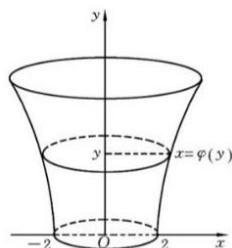
\includegraphics[width=0.42\linewidth]{image/0f77ad05e9d6568c3a0a15cfec33846af7726b08f4a8a36c74034f9dbafe7f81.jpg}\end{center}

\Q{6.5.9-90}{15数二}已知高温物体置于低温介质中, 任一时刻该物体温度对时间的变化率与该时刻物体和介质的温差成正比. 现将一初始温度为 $120^{\circ}C$ 的物体在 $20^{\circ}C$ 恒温介质中冷却, $30\mathrm{min}$ 后该物体温度降至 $30^{\circ}C$ , 若要将该物体的温度继续降至 $21^{\circ}C$ , 还需冷却多长时间。

\end{document}